\chapter[Design und Durchführung der Onlinebefragung]{Design und Durchführung der Onlinebefragung zur Kasusrektion von \object{wegen}, \object{während}, \object{dank}, \object{gegenüber} und \object{seit}}
\label{cha:Methode}
%\setlist[enumerate]{itemsep=-.5cm}
%\setlist[itemize]{itemsep=-9pt}
Mithilfe einer Onlineumfrage, an der 397 Sprachbenutzer:innen teilnahmen, wurden Daten zur metapragmatischen Reflexion über die Rektionsvarianten ausgewählter Sekundärpräpositionen sowie Daten zum Gebrauch und zur Akzeptabilität dieser Varianten erhoben. In diesem Kapitel wird das methodische Vorgehen bei der Onlinebefragung beschrieben. Dafür wird zunächst auf die Auswahl der getesteten Präpositionen, die Durchführung der Pretests und der Pilotstudie sowie die Verbreitung des Fragebogens eingegangen. Anschließend werden die einzelnen Teile des Fragebogens in der Reihenfolge vorgestellt, in der sie von den Befragten bearbeitet wurden. Schließlich wird beschrieben, welche Antworten von der Auswertung ausgeschlossen wurden und wie die Kategorisierung der Antworten auf offene Fragen erfolgte. 
Der komplette Fragebogen findet sich im digitalen Anhang.\footnote{Der Anhang zum vorliegenden Buch ist unter \url{https://osf.io/psv6h/?view_only=c1022edf82a74aab98616811ead6368a} abgelegt.}
\section{Konzipierung des Fragebogens}
\label{sec:Konzipierung}
Ziel des Fragebogens war es, ca. 200 bis 300 Sprecher:innen zu erreichen und sowohl ihre Sprachproduktion als auch ihre metapragmatische Reflexion abzufragen. Dafür wurde ein \textit{mixed methods}-Ansatz gewählt, indem sowohl verschiedene linguistische Befragungstypen wie bspw. Produktionsexperiment und Akzeptabilitätstest als auch offene und geschlossene Fragen kombiniert wurden (\autoref{sec:Methodologie}). 

Mit \object{Befragung zum Umgang mit Sprache} wurde für die Umfrage bewusst ein sehr allgemeiner Titel gewählt, der kaum Rückschlüsse auf den Untersuchungsgegenstand zulässt. Auch im Einladungstext, der zusammen mit der URL verschickt wurde, sowie im Begrüßungstext auf der ersten Seite des Fragebogens wird kaum etwas über den tatsächlichen Untersuchungsgegenstand preisgegeben (s. Fragebogen im digitalen Anhang). Die Teilnehmenden wurden zu Beginn des Fragebogens darauf hingewiesen, dass ihre Daten anonym behandelt werden und der Fragebogen einem wissenschaftlichen Forschungsinteresse dient. Es wurde kein Anreiz zur Teilnahme in Form einer Gewinnmöglichkeit o.\,Ä. gegeben. 

Die Fragen lassen sich in sechs Bereiche gliedern, aus denen sich die Umfrage in folgender Reihenfolge zusammensetzt: 
\begin{enumerate}
\item Abfrage der Sprachbewusstheit, der Einschätzung der eigenen Sprachkompetenz und der Variationstoleranz (\autoref{sec:RE})
\item Fragen zu persönlichen Zweifelsfällen (für die vorliegende Studie nicht relevant)
\item Produktionsexperiment bestehend aus zwei Lückentexten (\autoref{sec:LU})
\item Abfrage von Assoziationen mit den Rektionsvarianten (\autoref{sec:Ass})
\item Akzeptabilitätstest (\autoref{sec:Akz})
\item Abfrage von Metadaten (\autoref{sec:ME})
\end{enumerate}
Die unter 2 genannten Fragen zu persönlichen Zweifelsfällen wie \object{gewinkt/gewunken} oder \object{bin/habe gesessen} fließen nicht in die vorliegende Studie ein und werden hier daher nicht weiter besprochen.\footnote{Einige der in diesem Teil des Fragebogens erhobenen Daten wurden in \citet{Vieregge.2019b} ausgewertet.} 

Die Reihenfolge wurde so gewählt, dass die Befragten zunächst nicht wissen, um welches sprachliche Phänomen es bei der Untersuchung geht. Zudem empfiehlt etwa \citet[741]{PorstSept.1996}, \glqq daß eine Befragung mit spannenden, themenbezogenen und die Befragungsperson betreffenden, aber technisch einfach zu bearbeitenden Fragen beginnen\grqq{} sollte. 
Daher beantworten die Proband:innen im ersten Teil des Fragebogens Fragen zu ihrer Meinung über Sprache und zu ihrem Umgang mit Sprache. Im anschließenden Produktionsteil wird durch Distraktoren vom Untersuchungsgegenstand abgelenkt. 
Die Fragen nach Assoziationen mit den Rektionskasus erfordern eine direkte Gegenüberstellung der Varianten, wodurch der Untersuchungsgegenstand vielen Befragten bewusst geworden sein wird. 
Die Abfrage der Assoziationen vor dem Akzeptabilitätstest zu platzieren, war jedoch wichtig, um zu gewährleisten, dass die Assoziationen unvoreingenommen geäußert werden. Metadaten wie etwa Alter, Muttersprache(n) und Beruf wurden ganz am Ende des Fragebogens erhoben.

\begin{sloppypar}
Der Fragebogen wurde so konzipiert, dass nicht alle Befragten jede Frage bekommen: Bei der Abfrage der Assoziationen und beim Akzeptabilitätstest werden die Befragten per Zufallsprinzip in Gruppen eingeteilt. 
Jede Gruppe bekommt unterschiedliche Fragen. 
Dadurch können alle Aspekte abgefragt werden, während die Bearbeitungszeit für den Einzelnen dennoch möglichst kurz gehalten wird. 
\end{sloppypar}

Für diese Studie wurde bewusst eine Onlinebefragung statt einer Befragung in Papierform gewählt, da Onlineumfragen einige Vorteile gegenüber Papierfragebögen bieten. 
Zu diesen Vorteilen zählt etwa die leichte Verbreitung und die damit verbundene Möglichkeit, eine große Anzahl heterogener Teilnehmergruppen zu erreichen \citep[s.][77]{Potschke2009}. 
Für diese Untersuchung war es insbesondere wichtig, Teilnehmer:innen aus verschiedenen Regionen Deutschlands zu gewinnen, um nicht nur Antworten von Sprecher:innen einer Regionalsprache zu erhalten. 
\citet[78]{Potschke2009} weist außerdem darauf hin, dass bei Onlinebefragungen die Teilnahmebereitschaft höher ist als bei anderen Formen der Befragung (etwa bei Telefoninterviews). 
Ein weiterer wichtiger Vorteil ist die Möglichkeit, die Reihenfolge der Fragen zu randomisieren \citep[s.][109]{Baur2009}. 
So können eventuelle Reihenfolgeeffekte kontrolliert werden. 
Auch die oben erwähnte zufällige Gruppeneinteilung ist bei einem Onlinefragebogen deutlich leichter möglich als bei einem Fragebogen in Papierform. 
Zudem sind die online erhobenen Daten direkt in einem passenden Format verfügbar, was sowohl den Zeitaufwand reduziert als auch Übertragungsfehler vermeidet \citep[s.][77]{Potschke2009}.

Für die Onlinebefragung wurde mithilfe der frei zugänglichen Software SoSci Survey \citep[s.][]{Leiner2014} ein standardisierter Fragebogen erstellt und über den Server von SoSci Survey unter \url{https://www.soscisurvey.de/Umgang\_mit\_Sprache/} zugänglich gemacht.  

Bei der Konzipierung des Fragebogens waren mehrere Schritte nötig: Zunächst wurden vier Sekundärpräpositionen und eine Primärpräposition ausgewählt (\autoref{cha:AuswahlPraep}), anschließend wurde der Fragebogen in verschiedenen Pretests getestet und es wurde eine Pilotstudie durchgeführt (\autoref{sec:PretestPilot}). Danach wurde der Fragebogen noch einmal überarbeitet, bevor die endgültige Version für die tatsächliche Datenerhebung online gestellt wurde. Auf die einzelnen Schritte wird in den folgenden Abschnitten näher eingegangen. 

\subsection{Auswahl der Präpositionen} 
\label{cha:AuswahlPraep}
\largerpage
Bei der Auswahl der Sekundärpräpositionen, die im Fragebogen abgefragt werden, wurden zwei Kriterien berücksichtigt, wie \autoref{table:AuswahlPraep} zeigt. Das erste Kriterium bildet die ursprüngliche Rektion: Stand die Präposition ursprünglich mit Genitiv oder mit Dativ? Das zweite Kriterium bildet die ursprüngliche Stellung: Wurde die Präposition immer schon vorangestellt oder handelte es sich ursprünglich um eine Post- oder Zirkumposition? Durch die vier Präpositionen \object {während, wegen, dank} und \object {gegenüber} ist jede Kombination einmal vertreten. Die Kriterien wurden herangezogen, um zu überprüfen, welchen Einfluss der sprachhistorische Ausgangspunkt einer Präposition darauf hat, welche Indexikalitäten die Varianten heute aufweisen, mit welchem Kasus die Präposition von den Befragten gebraucht wird und inwiefern sich die Kasus in ihren Verwendungskontexten unterscheiden (zum genauen Ablauf der Entwicklung der einzelnen Präpositionen s. \autoref{sec:PraepDE}). 
Für die Frage nach der Bewertung der Rektionsvarianten reicht eine synchrone Perspektive zudem nicht aus, da die Stigmatisierung teilweise weit zurückreicht, wie in \autoref{sec:IndexikalitaetRektionskasushistorisch} gezeigt wurde.

\begin{table}
\centering
\begin{tabular}{lll}
\lsptoprule
                                           & ursprünglich & ursprünglich  \\
                                           & Genitivrektion & Dativrektion\\
\midrule
immer schon   präponiert                & \object{während}                              & \object{dank}                               \\
ursprünglich zirkum-   oder postponiert & \object{wegen}                                 & \object{gegenüber}                          \\
\lspbottomrule
\end{tabular}
\caption{Auswahl der Präpositionen}
\label{table:AuswahlPraep}
\end{table}

Bei der Präposition \object{wegen} spielte als drittes Kriterium neben der ursprünglichen Rektion und der ursprünglichen Position die soziolinguistische Salienz eine Rolle: Es wird angenommen, dass sich \object{wegen} von den anderen Präpositionen durch eine besonders hohe soziolinguistische Salienz der Rektionsvarianten unterscheidet (s.~\autoref{sec:MetapragmatischeBewusstheit}). 

Die Präposition \object{gegenüber} wurde ausgewählt, da sie in ihrer Rektion noch kaum schwankt und stark zum Dativ tendiert. Somit verhält sie sich anders als die stark schwankenden oder eher zum Genitiv neigenden Vertreter und eignet sie sich gut als Vergleichspunkt. 

Zusätzlich zu den vier Sekundärpräpositionen wurde die Primärpräposition \object{seit} in den Fragebogen aufgenommen. Dadurch soll überprüft werden, ob Befragte in bestimmten Fällen auch bei Primärpräpositionen den Genitiv wählen, die zwar eigentlich in ihrer Dativrektion stabil sind, bei denen die Genitivrektion aber dennoch vereinzelt beobachtet werden kann (\cites[s.][211]{DiMeola2009}[227]{DiMeola2011}; \autoref{sec:Differenzierung}). 


\subsection{Pretests und Pilotstudie}
\label{sec:PretestPilot}
\largerpage
\begin{sloppypar}
Während der Entwicklungsphase des Fragebogens wurden mehrere Pretests durchgeführt. Direkt nach der Erstellung des ersten Fragebogenentwurfs wurde ein Vortest mit sechs Proband:innen durchgeführt, um den Fragebogen zu überprüfen und gegebenenfalls zu überarbeiten. Nach einer ersten Überarbeitungsphase wurde anschließend bei drei Pretests die \textit{think-aloud}-Methode angewendet \citep[s.][194]{Porst2014}: Die Proband:innen wurden gebeten, während der Bearbeitung laut zu lesen und zu überlegen. Solche kognitiven Pretests ermöglichen Einblicke in die Verständlichkeit der Fragen und Anweisungen sowie in die Entscheidungsprozesse bei der Beantwortung der Fragen \citep[s.][195--196]{Porst2014}. Anschließend wurden erneut zwei Pretests ohne die \textit{think-aloud}-Methode durchgeführt. Diese dienten insbesondere der Überprüfung der benötigten Bearbeitungszeit. Außerdem wurde ein zusätzlicher Pretest für die im Fragebogen verwendeten Likertskalen durchgeführt, auf den in \autoref{sec:RE} eingegangen wird.
\end{sloppypar}

Nach den Pretests wurde ein technischer Funktionstest durchgeführt, um zu überprüfen, ob alle Fragen wie vorgesehen angezeigt werden, ob die eingebauten Zufallsgeneratoren funktionieren und ob alle Angaben korrekt gespeichert werden \citep[s.][]{Leiner2014}. 

Der nach den Pretests überarbeitete Fragebogen wurde zunächst in einer Pilotstudie getestet, die vom 05. August 2016 bis zum 11. August 2016 lief. An der Pilotstudie nahmen 46 Proband:innen teil, davon waren 31 weiblich und zwölf männlich, drei machten keine Angabe zu ihrem Geschlecht. Die Teilnehmer:innen waren zwischen 18 und 61 Jahre alt (Durchschnitt: 28 Jahre), die meisten (28 Personen) hatten mit einem Universitätsabschluss einen relativ hohen Bildungsstand. Zwei waren promoviert oder habilitiert, 13 hatten Abitur und drei Personen hatten einen Realschulabschluss. 

Im ersten Satz des Begrüßungstextes auf der ersten Seite des Fragebogens wurde nach dem ersten Tag, an dem der Fragebogen für die Pilotstudie online war, die Formulierung \object{im Rahmen einer Doktorarbeit zum Thema Grammatik} zu \object{in der Sprachwissenschaft des Deutschen} geändert. Da relativ viele Personen (30 von 40) den Fragebogen angeklickt und lediglich den Begrüßungstext gelesen hatten, wurde vermutet, dass die Erwähnung von Grammatik als Untersuchungsgegenstand abschreckend wirkt. Ein weiterer Grund für die relativ geringe Rücklaufstatistik am ersten Tag der Pilotstudie könnte die Ankündigung der Dauer von 15--20 Minuten gewesen sein.

Die Auswertung der Ergebnisse der Pilotstudie zeigten, dass an mehreren Stellen kleinere Überarbeitungen notwendig waren. So wurde nach der Pilotierungsphase etwa die Zufallsaufteilung in Gruppen verbessert. Die Assoziationen wurden in der Pilotstudie lediglich für die ursprünglichen Genitivpräpositionen \object{während} und \object{wegen} abgefragt. Hier wurde die Gruppenanzahl erhöht, um auch die Dativpräpositionen abzudecken. Auch im Akzeptabilitätstest wurde die Gruppeneinteilung verändert, sodass alle Präpositionen in einer informellen und in einer formellen Kondition abgefragt wurden. Außerdem wurde nach der Pilotstudie die Seitenaufteilung teilweise überarbeitet, um eine bessere Überprüfung der für eine Aufgabe benötigten Zeit zu ermöglichen. Die Bearbeitungszeit ist vor allem für den Ausschluss von Fällen mit auffällig langer oder auffällig kurzer Bearbeitungszeit relevant (s. \autoref{sec:Ausschluss}). 

Für das Produktionsexperiment war als ursprünglich postponierte Dativpräposition \object{gegenüber} ausgewählt worden. In den Pretests zeigte sich, dass einige Befragte Schwierigkeiten beim Ausfüllen der Lücken nach \object{gegenüber} hatten. Dies kann verschiedene Gründe gehabt haben, etwa, dass bei \object{gegenüber} neben Dativ- und Genitivrektion auch die Variante \object{gegenüber von X} möglich ist. Da \object{gegenüber} aufgrund seiner grammatischen Eigenschaften aber sehr gut für die Untersuchung geeignet ist, wurde die Präposition beibehalten und es wurden lediglich die Sätze, in denen \object{gegenüber} in den Lückentexten vorkommt, geändert.\footnote{Da vermutet wurde, dass die Rektion über \object{von} insbesondere im Falle einer lokalen Interpretation der Präposition möglich ist, wurde der Satz im informellen Lückentext so umformuliert, dass eine lokale Interpretation nicht mehr möglich ist: von \object{unser Tisch ist gegenüber \_\_\_(Haus) mit dem roten Tor} zu \object{ich hab jedenfalls keine Bedenken mehr gegenüber \_\_\_ (Plan)}. Im formellen Lückentext wurde das einzusetzende Element von einer Nominalphrase mit einer Substantivierung in ein einfaches Substantiv geändert: von \object{gegenüber \_\_\_ (Einarbeiten) in neue Tätigkeitsfelder bin ich stets aufgeschlossen} zu \object{wichtig ist mir insbesondere, Professionalität und Engagement gegenüber \_\_\_ (Beruf) zu zeigen}.} 
\section{Aufbau des Fragebogens}
\label{sec:Fragebogen}
Im folgenden Abschnitt geht es darum, wie der Fragebogen aufgebaut ist. Die einzelnen Teile und ihre Funktionen werden nacheinander vorgestellt. 
\subsection{Abfrage der Sprachbewusstheit, der Einschätzung der eigenen Sprachsicherheit und der Variationstoleranz}
\label{sec:RE}
\largerpage
Für die Bewertung der Rektionsvarianten durch die Befragten ist interessant, inwiefern sie sich als sprachinteressiert sehen, wie sicher sie sich in Bezug auf ihren Sprachgebrauch fühlen und wie offen sie gegenüber Variation in der Sprache sind. 
Daher werden die Sprachbewusstheit der Proband:innen, die Einschätzung der eigenen Sprachsicherheit und die Variationstoleranz der Proband:innen im Fragebogen abgefragt. 
Ziel dieser Abfragen ist eine Einteilung der Proband:innen nach folgenden Kriterien: sprachbewusst oder wenig sprachbewusst, hohe Einschätzung der eigenen Sprachsicherheit oder niedrige Einschätzung der eigenen Sprachsicherheit und eher präskriptiv oder variationstolerant. 
So kann später etwa überprüft werden, ob Personen, die eher präskriptiv eingestellt sind, anders mit grammatischer Variation umgehen als Personen, die Variation gegenüber offener sind. 

Für die Abfrage der Sprachbewusstheit, der Einschätzung der eigenen sprachlichen Sicherheit und der Variationstoleranz werden drei Likertskalen eingesetzt: Den Proband:innen werden Aussagen vorgelegt, zu denen sie auf einer fünfstufigen Skala (von 1 \glqq stimme gar nicht zu\grqq{} bis 5 \glqq stimme voll zu\grqq) ihre Zustimmung bzw. Ablehnung angeben müssen \citep[s.][62]{Rasinger2010}. 
Folgende Aussagen dienen im Fragebogen dazu, die Sprachbewusstheit der Proband:innen zu überprüfen: 
%\setlist[enumerate]{itemsep=-.5cm}
\begin{enumerate}
\item Ich denke häufig über die deutsche Sprache nach.
\item Mit dem Thema Sprache beschäftige ich mich nur sehr selten.
\item Ich interessiere mich für die deutsche Sprache. 
\end{enumerate}
%Warum diese? Literatur nennen? Oder Verweis auf \autoref{cha:Zweifelsfaelle}?
Diese Aussagen werden im Fragebogen auf einer Seite zusammen mit folgenden, die Einschätzung der eigenen Sprachsicherheit betreffenden Aussagen präsentiert: 
\largerpage
\begin{enumerate}
\item Wenn jemand eine Frage zu Grammatik oder Rechtschreibung hat, kann ich meistens weiterhelfen.
\item Ich bin bei sprachlichen Fragen häufig unsicher. 
\item Ich kenne mich gut mit der deutschen Grammatik aus.
\end{enumerate}
Auf der nächsten Fragebogenseite werden die Probend:innen gebeten, ihre Einschätzung zu folgenden Aussagen abzugeben, die sprachliche Normen und Normierung betreffen. 
So wird die Variationstoleranz der Proband:innen überprüft. 
\begin{enumerate}
\sloppy
\item Die deutsche Grammatik verfällt immer mehr. 
\item In der Sprache sollten feste Regeln vorschreiben, was richtig und was falsch ist. 
\item Es ist gut, dass sich der Duden dem aktuellen Sprachgebrauch anpasst. 
\item Je nach Region können verschiedene Sprachformen richtig sein. 
\end{enumerate}
Die Auswahl der zu bewertenden Aussagen enthält jeweils Aussagen, die die zu überprüfende Einstellung ablehnen, sowie solche, die sie befürworten. 

%Dabei geht es vor allem um das Aufdecken von Response-Sets, also von Mustern im Antwortverhalten der Proband:innen \cite[S.~275]{Gerich2010}. 
Bevor die für die Likertskalierung vorgesehenen Items Eingang in den Fragebogen finden, sind mehrere Schritte notwendig, um die Eignung der Items zu {tes\-ten}. \citet[1255]{Garrett2005} etwa betont, dass die Aussagen, die auf den Likertskalen bewertet werden sollen, idealerweise mithilfe einer Vorstudie zusammengestellt werden sollten, in der bspw. die Verständlichkeit überprüft wird. Anschließend sollte eine Itemanalyse durchgeführt werden \citep[s.][289]{Doring2016}. Bei der Itemanalyse geht es um die Ermittlung der Itemschwierigkeit, der Trennschärfe und der internen Konsistenz (Cronbachs Alpha, \citealp[s.][289]{Doring2016}). Diese Maße zeigen an, wie gut eine Likertskala tatsächlich geeignet ist, die zu überprüfende Variable zu testen.

Für die im Fragebogen eingesetzten Likertskalen wurden daher zunächst Sätze ausgewählt, mit denen die Einschätzung der eigenen Sprachsicherheit, die Sprachbewusstheit sowie die Variationstoleranz überprüft werden können. 
Diese Sätze wurden in den Pretests auf ihre Verständlichkeit und Beantwortbarkeit hin überprüft. 
Ungeeignete Items wurden umformuliert oder ersetzt (etwa zu komplexe Sätze wie \object{wenn es eine alte und eine neue Variante gibt, kann man in vielen Situationen beide verwenden}).
 
Anschließend wurden die übriggebliebenen bzw. umformulierten Sätze einer Itemanalyse unterzogen. 
Hierfür wurde 32 Testpersonen (davon ca. zwei Drittel Germanistikstudierende) nur der Ausschnitt des Fragebogens vorgelegt, der die Likertskalen enthält. 

Für die Abfrage der Sprachbewusstheit der Sprecher:innen und die Einschätzung der eigenen Sprachsicherheit wurden nur die oben genannten Sätze getestet. 
Um die Variationstoleranz der Sprecher:innen zu überprüfen, standen insgesamt sechs Sätze zur Verfügung, von denen mithilfe der Itemanalyse die vier besten ausgewählt wurden. 
Zusätzlich zu den oben genannten wurden folgende Items überprüft: 
\begin{enumerate}
\item[5.] Häufig gibt es in der Grammatik mehr als eine korrekte Variante.  
\item[6.] Man sollte am besten so sprechen, wie man auch schreiben würde. 
\end{enumerate}
Die Items, bei denen eine Zustimmung die Ablehnung des zu überprüfenden Konzepts hieße, müssen vor der Auswertung umgepolt werden, sodass der Wert fünf immer der vollen Zustimmung zum abgefragten Konzept (z.\,B. Sprachbewusstheit) entspricht (\cites[s.][242]{Diekmann2008}[75]{Rasinger2010}). 
Das trifft jeweils auf das zweite Item bei den Skalen für Sprachbewusstheit sowie Sprachsicherheit und auf Item eins, zwei und sechs der Skala zur Variationstoleranz zu. 
Nach dieser Umpolung wurden in R \citep[][Version 3.6.1]{RCoreTeam2019} mithilfe des Pakets psych \citep[][Version 2.0.7]{Revelle2016} Maße für die Trennschärfe, die Itemschwierigkeit und die Reliabilität berechnet.

Die Trennschärfe gibt an, wie gut ein einzelnes Item dazu geeignet ist, die Variablen\-aus\-prä\-gung widerzuspiegeln. 
Sie betrifft also \glqq das Ausmaß, zu dem ein einzelnes Item in der Lage ist, zwischen verschiedenen Ausprägungen der latenten Variable zu diskriminieren\grqq{}~\citep[275]{Gerich2010}. 
Im Falle der Skala für die Abfrage der Variationstoleranz etwa ist ein Item mit hoher Trennschärfe gut dazu geeignet, zwischen Personen mit deskriptiver Normauffassung und Personen mit präskriptiver Normauffassung zu differenziern. 
Dies wird anhand der Korrelation eines einzelnen Items mit dem Gesamtmittelwert aller Items ermittelt \citep[s.][289]{Doring2016}. 
Das heißt, dem Trennschärfekoeffizienten liegt die Annahme zugrunde, dass z.\,B. eine Probandin, die insgesamt auf der Skala den präskriptiven Aussagen eher zustimmt (hoher Gesamtmittelwert), auch einer einzelnen präskriptiven Aussage zustimmt (hoher Wert bei Einzelitem). 
Der Trennschärfekoeffizient liegt zwischen $-1$ (starke negative Korrelation) und 1 (starke positive Korrelation). 
Er sollte laut \citet[478]{Doring2016} mindestens 0,3 betragen und gilt ab einem Wert von 0,5 als hoch. 
Die Items fünf und sechs aus der Skala für die Variationstoleranz weisen mit 0,24 und 0,04 sehr geringe Trennschärfen auf und eignen sich daher nicht gut zur Trennung in Befragte, die Variation gegenüber offen sind, und Befragte, die Variation in der Sprache ablehnen. 
Sie müssen also eventuell ausgeschlossen werden. 
Alle Items der Skalen für die Einschätzung der eigenen Sprachsicherheit und die Sprachbewusstheit erreichen Trennschärfekoeffizienten von über 0,6 und korrelieren damit in hohem Maße mit dem Gesamtmittelwert aller Items der jeweiligen Skala. 
Sie sind also gut geeignet, um zwischen den jeweils abgefragten Ausprägungen zu unterscheiden. 

Der Zustimmungsgrad\footnote{In der Literatur wird dieses Maß häufig auch als Schwierigkeitsgrad oder Itemschwierigkeit bezeichnet, da es bei Leistungstests die Schwierigkeit einer Frage ausdrückt \citep[s.][476]{Doring2016}.} gibt an, wie leicht einem Item von den Proband:innen zugestimmt wird. Das Maß dafür ist der im Pretest erzielte Mittelwert des Items. 
Sowohl Items, denen kaum jemand zustimmt, als auch solche, denen alle Befragten zustimmen, ermöglichen keine Unterteilung der Befragten in z.\,B. solche mit geringer und solche mit hoher Variationstoleranz. 
Daher werden Items mit mittlerem Zustimmungsgrad bevorzugt \citep[s.][477]{Doring2016}. 
Hier wird davon ausgegangen, dass nicht alle Befragten zustimmen. %warum ist dann hier nicht die Standardabweichung total wichtig??
Für eine fünfstufige Skala entspricht ein mittlerer Zustimmungsgrad etwa Werten zwischen zwei und vier. 
Alle Items aus den Skalen zur Einschätzung der eigenen Sprachsicherheit und zur Sprachbewusstheit lagen im Pretest ungefähr in diesem Bereich (min. 3,6 und max. 4,1). 
Die Items, die die Offenheit für Variation überprüfen sollen, weisen höhere Zustimmungsgrade auf. 
Die Werte der Items \object{Es ist gut, dass sich der Duden dem aktuellen Sprachgebrauch anpasst} und \object{Man sollte am besten so sprechen, wie man auch schreiben würde} liegen dabei bei über vier. 
Da letzteres Item bereits aufgrund seiner geringen Trennschärfe ausgeschlossen werden muss, bleibt lediglich ein hoher Zustimmungsgrad für Item drei bestehen, das heißt, die Aussage \object{Es ist gut, dass sich der Duden dem aktuellen Sprachgebrauch anpasst} wurde im Pretest selten abgelehnt. 
Dies entspricht einer hohen Zustimmungsrate zur Variationstoleranz bei diesem Item. 
Dass Variation im Pretest selten abgelehnt wurde, liegt wahrscheinlich vor allem daran, dass überwiegend Germanistikstudierende befragt wurden, die sich deskriptiv mit Sprache beschäftigen. 
Für die spätere Befragung können daher geringere Zustimmungsgrade erwartet werden, sodass das Item für die Datenerhebung beibehalten wird. %Das Item kann außerdem deshalb als geeigneter Indikator eingestuft werden, da sich in einer vorigen Untersuchung von Forenbeiträgen gezeigt hat, dass eine Ablehnung der Anpassung des Dudens an den Sprachgebrauch meist mit einer präskriptiven Einstellung einhergeht (wie darauf verweisen?). 

\begin{sloppypar}
Zur Überprüfung der Reliabilität wurde die interne Konsistenzprüfung gewählt \citep[s.][467--469]{Doring2016}. 
Das Maß dafür ist Cronbachs Alpha.\footnote{Cronbachs Alpha ist teilweise umstritten, da es dazu neigt, die Reliabilität eines Tests zu überschätzen. Dennoch wird hier darauf zurückgegriffen, da es sich um \glqq das mit Abstand gebräuchlichste Reliabilitätsmaß\grqq{}~\citep[444]{Doring2016} handelt, was die Angabe gut vergleichbar macht, und da diese Methode stabilere Ergebnisse liefert als die alternative Testhalbierungsmethode \citep[s.][467]{Doring2016}.} 
%\begin{quote}{Die Interne Konsistenz-Methode ist eine Verallgemeinerung der Testhalbierungs-Methode. Anstatt den hinsichtlich seiner Messgenauigkeit zu pr{\"u}fenden Test willk{\"u}rlich in zwei H{\"a}lften einzuteilen, wird er in seine einzelnen Items aufgeteilt und es werden alle bivariaten Korrelationen zwischen den Items berechnet und gemittelt. Die Interne Konsistenz wird typischerweise mit dem Cronbach Alpha-Koeffizienten berechnet. Er ist das mit Abstand gebr{\"a}uchlichste Reliabilit{\"a}tsma{\ss}.}~\cite[S.~444]{Doring2016}\end{quote}
Als ausreichend gelten Reliabilitätskoeffizienten von über 0,8 \citep[s.][443]{Doring2016}. 
Allerdings können auch Skalen mit niedrigeren Cronbachs Alpha-Werten zum Einsatz kommen. 
Cronbachs Alpha ist unter anderem von der Anzahl der Items in einer Skala abhängig, deshalb werden, um einen Fragebogen möglichst kurz zu halten, auch Reliabilitätsmaße, die etwas unter 0,8 liegen, akzeptiert \citep[s.][444]{Doring2016}. 
Zu berücksichtigen ist außerdem, dass die Messung von Einstellungen schwieriger ist als bspw. die Messung von Leistung, sodass auch dies geringere Cronbachs Alpha-Werte rechtfertigt \citep[s.][444]{Doring2016}. 
Die Skalen zur Messung der Einschätzung der eigenen Sprachsicherheit sowie der Sprachbewusstheit weisen beide Reliabilitätswerte von über 0,8 auf und können damit als ausreichend reliabel gelten (Cronbachs Alpha = 0,81 und 0,87). 
Für die Skala zur Messung der Variationstoleranz liegt Cronbachs Alpha nur bei 0,64 und ist somit zu niedrig. 
Um einen akzeptablen Wert von 0,71 zu erhalten, müssen die Items fünf und sechs ausgeschlossen werden. 
\end{sloppypar}

Die Itemanalyse im Pretest hat gezeigt, dass die Skalen zur Einschätzung der eigenen Sprachkompetenz und zur Sprachbewusstheit in der Datenerhebungsphase so bestehen bleiben können. Die Skala, die Aufschluss über die Variationstoleranz der Proband:innen geben soll, muss auf vier Items reduziert werden. Ausgeschlossen werden die Items fünf und sechs (\object{häufig gibt es in der Grammatik mehr als eine korrekte Variante} und \object{man sollte am besten so sprechen, wie man auch schreiben würde}).
%\subsection{Fragen zu persönlichen Zweifelsfällen}
%\label{sec:persZF}
%In dem Teil zu eigenen Zweifelsfällen und dem Umgang mit diesen wurden die Proband:innen zunächst in einer offenen Frage gebeten, sprachliche Phänomene zu nennen, bei denen sie häufig in Zweifel geraten (\glqq Bei welchen sprachlichen Phänomenen zweifeln Sie immer wieder, welche Variante Sie verwenden sollten?\grqq). Diese offene Frage wurde bewusst relativ am Anfang des Fragebogens platziert, damit die Befragten unvoreingenommen die Zweifelsfälle nennen, die ihnen zuerst einfallen. Um die Aufgabe zu erleichtern und Antworten zu vermeiden, die zu weit von möglichen Zweifelsfällen wegführen, findet sich unter der Frage ein Hinweis mit zwei Beispielen für Zweifelsfälle. Dabei wurden die Befragten mithilfe eines Zufallsgenerators auf drei Gruppen aufgeteilt, sodass die eine Gruppe Beispiele aus dem Bereich der orthografischen Zweifelsfälle bekam (\object{Delfin} oder \object{Delphin} und \object{seit} oder \object{seid}), eine zweite Gruppe morphologische Zweifelsfälle aus dem Bereich der Verbalflexion (\object{schwamm} oder \object{schwomm} und \object{gehängt} oder \object{gehangen}) und eine dritte morphosyntaktische Zweifelsfälle (\object{dem Abkommen entsprechend} oder \object{entsprechend dem Abkommen} und \object{Ende diesen Jahres} oder \object{Ende dieses Jahres}). Die Frage nach den persönlichen Zweifelsfällen wurde alleine auf einer Seite platziert, sodass später anhand der Verweildauer auf der Seite zu sehen war, wie lange die Befragten hier überlegten.\\
%An die erste Frage zu den persönlichen Zweifelsfällen schloss sich im Fragebogen eine Seite mit weiteren Fragen dazu an. Hier sollten die Befragten Auskunft über die Situationen geben, in denen bei ihnen sprachliche Zweifel aufkommen können. Für jede Situation konnte zwischen \glqq ja\grqq, \glqq nein\grqq{} und  \glqq in dieser Situation bin ich fast nie\grqq{} ausgewählt werden. Folgende Situationen standen zur Auswahl: 
%\begin{itemize}
%\item beim Verfassen von formellen Briefen (z.\,B. Bewerbungen)
%\item beim Lesen von formellen Briefen 
%\item beim Verfassen beruflicher E-Mails 
%\item beim Lesen beruflicher E-Mails 
%\item beim Schreiben privater E-Mails 
%\item beim Lesen privater E-Mails 
%\item beim Schreiben privater SMS, Whats-App- oder Facebook-Nachrichten
%\item beim Lesen privater SMS, Whats-App- oder Facebook-Nachrichten
%\item beim Lesen literarischer Texte
%\item beim Lesen von Pressetexten
%\item beim Hören/Sehen von Nachrichtensendungen 
%\item in privaten Gesprächen 
%\item in offiziellen Gesprächen (z.\,B. Bewerbung, Arzt, Amt)
%\item in einer anderen Situation  
%\end{itemize}
%Bei der Auflistung der Situationen, in denen möglicherweise Zweifel aufkommen, wurde lexikalisch zwischen eher formellen Kontexten und eher informellen Kontexten differenziert, indem zum Beispiel \object{beim \textbf{Verfassen} beruflicher E-Mails}, aber \object{beim \textbf{Schreiben} privater E-Mails} aufgeführt wurde. \\
%Die Proband:innen wurden außerdem danach gefragt, wie häufig sie generell über sprachliche Fragen in Zweifel geraten (\glqq nie\grqq , \glqq selten\grqq, \glqq ab und zu\grqq, \glqq häufig\grqq oder \glqq keine Angabe\grqq). In der letzten Frage zu den persönlichen Zweifelsfällen wurde abgefragt, wie sich die Untersuchungsteilnehmer:innen in Situationen des Zweifelns helfen, etwa wo sie nachschlagen. Hier wurde bewusst eine offene Frage gestellt, bei der auch mehrere Antworten gegeben werden konnten. 
\subsection{Produktionsexperiment} 
\label{sec:LU}
Das Produktionsexperiment soll überprüfen, für welche Rektionsvariante sich Sprecher:innen in zwei verschiedenen Kontexten entscheiden. 
Der Produktionsteil besteht aus einem Lückentext mit als informell registrierten sprachlichen Formen und einem zweiten Lückentext mit als formell registrierten sprachlichen Formen (zur Registrierung s. \autoref{sec:Indexikalitaet}). 
Der informelle Text ist einer elektronischen Textnachricht oder E-Mail nachempfunden. 
Er enthält zahlreiche Mündlichkeitsmarker wie Apokopen und Ellipsen und ist auch in seiner Lexik (\object{drangehen, nix, sauer}) informell gehalten, da dieser Bereich besonders stark registriert ist \citep[s.][88]{Halliday1964}. 
Zudem weist der Text ein Emoticon auf. 
Der zweite Lückentext hingegen stellt ein fiktives Bewerbungsschreiben an eine Unternehmensberatung dar und ist somit einem sehr formellen Register zuzuordnen. 
Die Textsorten wurden so ausgewählt, dass sie sich möglichst stark in der ihnen zugeschriebenen Formalität unterscheiden.  
Die Reihenfolge, in der die beiden Lückentexte präsentiert werden, ist randomisiert. So sollen mögliche Reihenfolgeeffekte überprüft werden \citep[s.][37--38]{Porst2014}. 
% Änderung Anfang! 
Als wie formell die Lückentexte tatsächlich wahrgenommen werden, wurde in einer kurzen zusätzlichen Umfrage getestet (s. \autoref{sec:FormLU}).
% Änderung Ende!

\begin{sloppypar}
Die Aufgabe % Änderung Anfang 
im Produktionsexperiment ist jeweils, das Substantiv, das in Klammern hinter der Lücke nach der Prä\-po\-si\-tion steht, mit der passenden Form des Definitartikels und eventuell der Geni\-tiv\-end\-ung in die Lücke einzutragen. Die Anweisung für die Proband:innen lautet: 
\end{sloppypar}

\begin{quote}\glqq Bitte vervollständigen Sie nun die folgenden Lückentexte, indem Sie jeweils den Artikel und das Substantiv in der richtigen Form in die Lücke eintragen (siehe Beispiel). Verwenden Sie immer nur den bestimmten Artikel (\object{der, die, das} etc). Gehen Sie dabei bitte möglichst intuitiv vor -- schlagen Sie nicht im Internet oder im Wörterbuch nach.\grqq{}\end{quote}

Ein Beispiel zeigt das Vorgehen (s.~\autoref{pic:BspLUE}). In beiden Lückentexten sind alle vier untersuchten Sekundärpräpositionen enthalten: \object{wegen, während, gegenüber} und \object{dank}. Zusätzlich kommt in beiden Lückentexten die Primärpräposition \object{seit} vor. So soll überprüft werden, ob Testpersonen auch bei Primärpräpositionen in formellen Kontexten hin und wieder den Genitiv wählen.

\begin{figure}
\centering
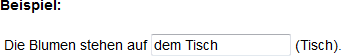
\includegraphics[scale=0.8]{BspLueckentextBlumen}
\caption{Beispiel zum Ausfüllen der Lückentexte}
\label{pic:BspLUE}
\end{figure}

Die Substantive in den relevanten Präpositionalphrasen wurden so gewählt, dass sie im Genitiv keine nennenswerte Schwankung zwischen langer und kurzer Endung (oder gegebenenfalls auch der Nullendung) aufweisen, also nicht zu Zweifeln oder Unsicherheiten führen \citep[zu Zweifelsfällen bei Genitivendungen s. etwa][]{Szczepaniak2014}. Die mögliche Zeichenzahl in den Lücken wurde jeweils so definiert, dass der Eintrag mindestens die Länge der Dativform mit Definitartikel (z.\,B. \object{dem Verkauf}) und maximal die Länge der Genitivform mit Definitartikel und langer Endung (z.\,B. \object{des Verkaufes}) haben kann. 

Als Distraktoren wurden Fremd- und Lehnwörter mit Genusschwankungen gewählt (\object{Annonce, Go-Live, Blog, Laptop, Event}). Diese eigneten sich gut, da die Proband:innen auch in diesen Fällen überlegen müssen, welchen Artikel sie einsetzen. So lenken die Distraktoren die Aufmerksamkeit weg von der Rektion der Präpositionen hin zur Wahl des Genus. Damit liegt aus der Perspektive der Befragten der Fokus auf der Auswahl einer Form des Definitartikels und nicht nur auf Kasusunterschieden. 
\subsection{Assoziationen als Hinweis auf Indexikalitäten} 
\label{sec:Ass}
Die Frage nach möglichen Assoziationen zu den Rektionsvarianten soll zeigen, welche Indexikalitäten den Varianten von den Befragten zugeschrieben werden (zur Indexikalisierung der Varianten s. \autoref{sec:IndexikalitaetRektionskasus}). 
Hier werden den Proband:innen zwei Versionen eines Satzes präsentiert, die sich ausschließlich in der Rektion der enthaltenen Präposition unterscheiden. 
Damit wird ein indirekter Ansatz (\textit{indirect approach}) gewählt, bei dem nicht nach der Einstellung zu einer vordefinierten Kategorie gefragt wird (etwa \object{was denken Sie über den Dativ?}), sondern bei dem mit Stimuli gearbeitet wird~\citep[s.][1251--1252]{Garrett2005}. 

Die Assoziationsabfrage steht bewusst nach dem Produktionsteil, damit die Proband:innen noch nicht für die Kasusvariation sensibilisiert worden sind, wenn sie die Lückentexte ausfüllen.
Mithilfe eines Zufallsgenerators werden die Teilnehmenden bei der Assoziationsabfrage auf vier Gruppen verteilt. 
Jede Gruppe erhält nur ein Satzpaar mit einer der vier Präpositionen. 
So kann die Fragebogenlänge reduziert und dennoch jede der vier Präpositionen abgefragt werden. 
Die Sätze zu den abgefragten Präpositionen sind folgende: 

\ea 
\ea  Ich bin wegen dem Starkregen zu spät gekommen.
\ex  Ich bin wegen des Starkregens zu spät gekommen.
\z 
\ex
\ea Während dem Telefonat mache ich Notizen.
\ex  Während des Telefonats mache ich Notizen.
\z 
\ex
\ea Dank des Brückentags konnte ich ihn besuchen.
\ex Dank dem Brückentag konnte ich ihn besuchen.
\z 
\ex
\ea Sie hat es gegenüber des Lehrers nicht erwähnt.
\ex Sie hat es gegenüber dem Lehrer nicht erwähnt.
\z
\z
Die Befragten werden zunächst gebeten, mögliche Assoziationen zur ersten Variante des präsentierten Satzes zu äußern. Anschließend werden sie nach Assoziationen zur zweiten Satzvariante gefragt. Die Assoziationen können jeweils frei in ein Textfeld eingetragen werden. Die Frage ist offen gehalten (bspw. \glqq welche Assoziationen haben Sie zu Variante~1 (\object{Sie hat es gegenüber des Lehrers nicht erwähnt.})? Bitte notieren Sie, was Ihnen spontan dazu einfällt.\grqq), um keine mögliche Assoziation auszuschließen oder erst hervorzurufen (\autoref{sec:Methodologie}). Die Gestaltung als offene Frage ist hier auch deshalb wichtig, da offene Fragen \glqq den Befragungspersonen die Möglichkeit bieten, so zu sprechen, wie sie es gewohnt sind\grqq{} \citep[s.][739]{PorstSept.1996}. So soll festgestellt werden, ob eine mögliche Indexikalisierung der Varianten Teil des metasprachlichen Wissens der Befragten über die Rektionsvarianten der Präpositionen ist. Ein Nachteil bei offenen Fragen kann sein, dass sie durch eine große Zahl an Antwortkategorien schwer auszuwerten sind, weshalb sie möglichst fokussiert formuliert sein sollten (\citealp[s.][62--63]{Porst2014} sowie \autoref{sec:Methodologie}). Um Nennungen von Assoziationen, die sich nicht auf den Rektionskasus beziehen, möglichst gering zu halten, wurden im Fragebogen deshalb jeweils Satzpaare präsentiert, die sich nur im Kasus der von der Präposition regierten Nominalphrase unterscheiden. 

Schon die Vorgabe einer Anzahl, wie viele freie Nennungen gemacht werden sollen, sehen \citet[216]{Garrett.2004} eher als Nachteil für die Auswertung. 
Tatsächlich kann es interessant sein, sich anzusehen, wie produktiv die Befragten beim Antwortengeben sind~\citep[s.][71]{Adler.2018}. 
Daher wurden den Befragten hier beliebig viele Felder zur Verfügung gestellt. 

Zusätzlich zu den freien Assoziationen wurde abgefragt, inwiefern Proband:innen Personen, die die Variante mit Dativrektion bzw. die Variante mit Genitivrektion äußern, bestimmte Eigenschaften wie z.\,B. \glq gebildet\grq{} zuschreiben. Dies wurde mithilfe semantischer Differenziale (auch \object{Polaritätsprofile} genannt) überprüft (\cites[s.][1255]{Garrett2005}[234]{Atteslander2010}; \autoref{sec:Methodologie}). Bei dieser Methode werden den Befragten mehrere gegensätzliche Eigenschaftspaare präsentiert, die \glqq zu dem Objekt in keinem unmittelbaren sachlichen, jedoch in einem assoziativen Bezug\grqq{} \citep[234]{Atteslander2010} stehen  und die jeweils die Pole einer Skala bilden. In der vorliegenden Untersuchung sollen die Befragten die Rektionsvarianten auf fünfstufigen Skalen zwischen ungebildet~--~gebildet, unsympathisch~--~sympathisch, inkompetent~--~kompetent und unfreundlich~--~freundlich einordnen (s. \autoref{pic:SemDiffSc}). 
Laut \citet[49]{Preston2004} sind sozialer Status und Sympathie die wichtigsten Bewertungsaspekte für sprachliche Varianten (\autoref{sec:Bewertungsgrundlage}), weshalb sie auch hier herangezogen wurden. Die Kombination aus freien Assoziationen und semantischen Differenzialen ermöglicht es, sowohl mögliche unerwartete Antworten zu bekommen als auch die bereits bestehende Hypothese zu überprüfen, dass sich die Varianten in der Bewertung unterscheiden, was sozialen Status und Sympathie angeht.  

\begin{figure}
\centering
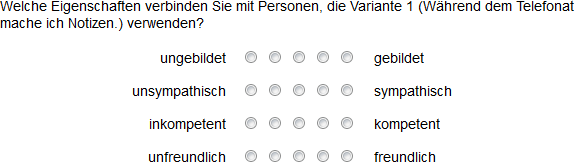
\includegraphics[scale=0.8]{SemDiffSc}
\caption{Semantische Differenziale zu den Rektionsvarianten}
\label{pic:SemDiffSc}
\end{figure}

\subsection{Akzeptabilitätstest} 
\label{sec:Akz}
Der Akzeptabilitätstest besteht aus zwei Teilen, die auf zwei Seiten des Fragebogens aufgeteilt sind. 
Im ersten Teil werden die Proband:innen gebeten, sich eine Situation vorzustellen, die ein formelles Register erfordert: \glqq Stellen Sie sich vor, Sie korrigieren einen förmlichen Brief an ein Amt, den ein guter Freund geschrieben hat. 
Wie würden Sie die sprachliche Form der folgenden Formulierungen bewerten?\grqq{} Im zweiten Teil hingegen erfordert die beschriebene Situation ein eher informelles Register: \glqq Stellen Sie sich vor, Sie unterhalten sich mit einem guten Freund. 
Wie würden Sie die sprachliche Form der folgenden Formulierungen bewerten?\grqq{} 
Wie \citet[182]{Koplenig.2016} zeigen, weisen förmliche Schreiben und Gespräche mit Freunden recht große Unterschiede auf, was die Akzeptabilität von Varianten angeht, die nicht dem geschriebenen Standard zuzuordnen sind. 
Diese Situationen wurden daher gewählt, um die Registrierung der Rektionsvarianten zu überprüfen.

Der Akzeptabilitätstest erfolgt nach der Assoziationsabfrage, damit die Befragten bei der Frage nach möglichen Assoziationen noch nicht von den im Akzeptabilitätstest vorgegebenen Registerunterschieden (formell und informell) beeinflusst werden und ihre Assoziationen möglichst frei äußern können. 

Die Befragten werden für den Akzeptabilitätstest erneut per Zufallsgenerator in vier Gruppen eingeteilt. 
Die Gruppen 1 und 3 bekommen Beispiele mit ursprünglichen Dativpräpositionen, die Gruppen 2 und 4 Beispiele mit ursprünglichen Genitivpräpositionen. 
Die Gruppen 1 und 3 bzw. 2 und 4 unterscheiden sich untereinander darin, welche Präposition in welcher Kondition vorkommt. 
\begin{description}
\item Gruppe 1\\ formeller Teil: \object{gegenüber des Sachbearbeiters}\\ informeller Teil: \object{dank des Urlaubs}
\item Gruppe 2\\ formeller Teil: \object{während dem Vortrag}\\ informeller Teil: \object{wegen dem Urlaub}
\item Gruppe 3\\ formeller Teil: \object{dank des Sachbearbeiters}\\ informeller Teil: \object{gegenüber des Schaffners}
\item Gruppe 4\\ formeller Teil: \object{wegen dem Konto}\\ informeller Teil: \object{während dem Spiel}
\end{description}
Alle Beispiele weisen die jeweils neue, von der ursprünglichen Rektion abweichende Variante auf. 
Es wurde darauf geachtet, dass die Beispiele lexikalisch und semantisch in das jeweilige Setting passen. 
Zusätzlich wurden Distraktoren eingebaut, die sich in den Gruppen nicht unterschieden (z.\,B. \object{Herr Schulzes Geburtstag}). 
In jeder Gruppe wurde außerdem in beiden Konditionen \object{seit} mit Genitivrektion abgefragt:
\begin{description}
\item Alle Gruppen\\ formeller Teil: \object{seit des Sturms}\\ informeller Teil: \object{seit des Festes}
\end{description}
Wie bereits im Produktionsexperiment (\autoref{sec:LU}) dient die Primärpräposition zur Überprüfung der Hypothese, dass auch Primärpräpositionen in bestimmten Kontexten von einigen Sprachbenutzer:innen mit Genitivrektion akzeptiert werden. 
Da davon ausgegangen wurde, dass \object{seit} mit Genitivrektion besonders salient ist, ist dieses Beispiel jeweils das letzte in einem Setting. 

Zu jedem Beispiel werden die Befragten gebeten, zunächst die Korrektheit sowie die Angemessenheit zu bewerten. 
Bei der Korrektheit können sie zwischen \glqq richtig\grqq{} und \glqq falsch\grqq{} entscheiden, bei der Angemessenheit zwischen \glqq in einem förmlichen Brief angemessen\grqq{} und \glqq in einem förmlichen Brief unangemessen\grqq{} bzw. zwischen \glqq in einem Gespräch angemessen\grqq{} und \glqq in einem Gespräch unangemessen\grqq. 
Geben sie an, dass etwas unangemessen ist, so müssen sie in einem Eingabefeld deutlich machen, warum sie es nicht akzeptieren. Auch hierfür wird eine offene Frage verwendet (\glqq was stört Sie?\grqq). 
Des Weiteren wird abgefragt, ob die Proband:innen die im Beispiel präsentierte Form selbst verwenden würden (\glqq würde ich selber schreiben/sagen\grqq) und wie sicher sie sich bei ihrer Antwort sind (\glqq ganz sicher, ziemlich sicher, etwas unsicher, sehr unsicher\grqq). 
Die Frage nach der eigenen Unsicherheit wurde in \citet{Vieregge.2019b} ausgewertet und wird in der vorliegenden Studie nicht weiter berücksichtigt. 

Mit diesem Testdesign können Daten zu mehreren Fragen erhoben werden: Beurteilen die Befragten eine Rektionsvariante generell als korrekt oder empfinden sie sie als Fehler? 
Wie sind die Varianten registriert? 
Wird die Korrektheit einer Variante anders bewertet als ihre Angemessenheit? 
Schreiben die Proband:innen die Verwendung der Varianten lediglich anderen zu oder sehen sie sie auch bei sich selbst? 
Gibt es Unsicherheiten bei der Bewertung der präsentierten Varianten? 
Dass sowohl im Akzeptabilitätstest als auch bei den Assoziationen und im Produktionstest nach konkreten Beispielen der ausgewählten Präpositionen mit Definitartikel und direkt darauf folgendem Substantiv gefragt wird, gewährleistet die Vergleichbarkeit zwischen den drei Fragebogenteilen und damit zwischen Bewertung und Produktion der Varianten. 
Für einen solchen Vergleich ist aufgrund des komplexen Verhältnisses von Einstellungen und Verhalten (\autoref{sec:Spracheinstellungsforschung}) zudem  wesentlich, dass die Erhebung der Einstellung und die Erhebung des Verhaltens (in diesem Fall der Produktion) in folgenden Punkten übereinstimmen \citep[s.][219]{Jonas.2014}: a) Welches Verhalten wird abgefragt (hier: Verwendung des Rektionskasus)? b) Was ist das Objekt des Verhaltens (hier die konkrete Präposition)?, c) In welcher Umgebung wird das Verhalten ausgeführt (hier formelle oder informelle Kondition)? d) In welchem Zeitrahmen wird das Verhalten ausgeführt (im Fragebogen beziehen sich die Fragen immer auf die Gegenwart)?

\subsection{Erhobene Metadaten}
\label{sec:ME}
\largerpage
\begin{sloppypar}
Im letzten Teil des Fragebogens werden personenbezogene Daten erhoben. Dazu gehören zunächst die Muttersprache(n) sowie die Region, in der eine Person größtenteils aufgewachsen ist. 
Nach den Muttersprachen wird mit folgender Formulierung gefragt: \glqq Welche Sprache(n) haben Sie als Muttersprache(n) erlernt (abgeschlossener Spracherwerb vor dem 12. Lebensjahr)?\grqq{} Die Herkunftsregion kann über ein Dropdown-Menü ausgewählt werden. Zur Verfügung stehen folgende Antwortmöglichkeiten: \glqq Norddeutschland (Hamburg, Niedersachsen, Schleswig\hyp Holstein, Bremen)\grqq, \glqq Süddeutschland (Bayern, Baden\hyp Württemberg)\grqq, \glqq Ostdeutschland (Berlin, Brandenburg, Mecklenburg\hyp Vorpommern, Sachsen, Thüringen, Sachsen\hyp Anhalt)\grqq, \glqq Westdeutschland (Nordrhein\hyp Westfalen, Rheinland\hyp Pfalz, Saarland, Hessen)\grqq, \glqq Österreich\grqq, \glqq Schweiz\grqq{} oder \glqq in einem anderen Land\grqq. 
% Änderung Anfang
Die Kategorien Ost und West umfassen damit auch Bundesländer, die ebenso den nördlichen bzw. südlichen Bundesländern hätten zugeordnet werden können (etwa Mecklenburg-Vorpommern oder das Saarland). 
Dies ist der Annahme geschuldet, dass aufgrund der Verbreitung des Fragebogens besonders viele Teilnehmende aus dem Norden (Hamburg, Schleswig-Holstein) und Süden (Bayern und Baden-Württemberg) stammen und die Gruppen bei einer anderen Zuordnung sehr ungleich besetzt wären.
Da ein Vergleich der Gruppen Nord und Süd angestrebt wurde, war zudem vor allem die klare Abgrenzung dieser beiden Regionen wichtig. 
\end{sloppypar}
% Änderung Ende

Ob eine Person einen Dialekt spricht, wird mithilfe einer offenen Frage überprüft: \glqq Wenn Sie in Ihrer Familie, mit Freunden oder in anderen Situationen einen Dialekt sprechen, nennen Sie diesen bitte.\grqq{} %Begründung/Problematisierung\\

Des Weiteren werden Daten zu Bildungsstand und Beruf erbeten. 
Die Befragten können den höchsten von ihnen erzielten Bildungsabschluss über ein Dropdown\hyp Menü auswählen. 
Die Auswahlmöglichkeiten sind hier bewusst zunächst recht ausdifferenziert, sodass die Befragten später zu Gruppen zusammengefasst werden können, ohne dass die genaue Information zur Art ihres Abschlusses verloren geht. 
Bei der Frage nach ihrem Beruf wurden die Befragten gebeten, möglichst genaue Angaben zu machen (\glqq Machen Sie gerne möglichst genaue Angaben, etwa \glq Lehrerin für Mathematik und Chemie\grq{} statt nur \glq Lehrerin\grq [...]\grqq). 
Zusätzlich wurden die Proband:innen gefragt, wie häufig sie im Beruf längere Texte wie z.\,B. Protokolle oder Artikel verfassen oder lesen. 
Hier konnte auf einer fünfstufigen Skala eine Antwortmöglichkeit zwischen \glqq ich verfasse oder lese im Beruf täglich längere Texte\grqq{} und \glqq ich verfasse und lese im Beruf nie längere Texte\grqq{} gewählt werden. 
Diese Daten sind wichtig, um etwa Zusammenhänge zwischen der beruflichen Tätigkeit und der Akzeptabilität oder zwischen dem Bildungsstand und der Produktion zu überprüfen. 

Die im Fragebogen zuletzt abgefragten Metadaten sind das Alter und das Geschlecht. Das Alter lässt sich von den Befragten in ein offenes Feld eintragen, sodass Altersgruppen in einem späteren Schritt gebildet werden können. Bei der Frage nach dem Geschlecht stehen die Antwortmöglichkeiten \glqq weiblich\grqq, \glqq männlich\grqq{} und \glqq anderes\grqq{} zur Auswahl. Abschließend besteht auf der letzten Fragebogenseite die Möglichkeit, Anmerkungen zu machen (\glqq Damit sind wir fast am Ende der Befragung angelangt. Falls Sie noch Anmerkungen zu der Umfrage haben, ist hier Platz dafür.\grqq). 
%Ein Rückschluss darauf, aus welcher Gruppe ein Datensatz stammt, ist über die Variable "{}Referenz"{} möglich. Die den verschiedenen Gruppen zur Verfügung gestellten URLs weisen unterschiedliche Markierungen auf, die als Referenz im Datensatz gespeichert werden. Zum Beispiel Ref=1 für die Fragebögen, die über die in der Facebookgruppe der Studienstiftung des deutschen Volkes geteilte URL aufgerufen wurden. 

\section{Datenerhebung und Aufbereitung der Daten}
\label{sec:DatenerhebungundAufbereitung}
Der Fragebogen war vom 18.01. bis 01.03.2017 online, also insgesamt 42 Tage. Zusätzlich erfolgte eine 25-tägige Nacherhebung vom 25.07. bis 19.08.2017. 

Die erhobenen Daten konnten als csv-Datei vom Server heruntergeladen werden. Im Datensatz wurden zusätzlich zu den Antworten automatisch weitere Variablen gespeichert. Zu nennen sind hier die Fallnummer, Datum und Uhrzeit des Fragebogenaufrufs, die Bearbeitungszeit der einzelnen Seiten, die Bearbeitungszeit des kompletten Fragebogens und der Anteil der fehlenden Antworten. Das Datenset wurde mithilfe von R \citep[][Version 3.6.1]{RCoreTeam2019} und RStudio \citep[][Version 1.2.5033]{RStudio.2019} aufbereitet und ausgewertet.\footnote{Folgende Pakete wurden verwendet: 
reshape \citep[][Version 0.8.8]{Wickham.2018}, 
readr \citep[][Version 1.3.1]{Wickham.2018b},
stringr \citep[][Version 1.4.0]{Wickham.2019}, 
tidyverse \citep[][Version 1.3.0]{Wickham.2019b},
ggbeeswarm \citep[][Version 0.6.0]{Clarke.2017}, 
rockchalk \citep[][Version 1.8.144]{Johnson.2019},
psych \citep[][Version 2.0.7]{Revelle2016},
party \citep[][Version 1.3-4]{Hothorn.2010},
Hmisc \citep[][Version 4.4-0]{Harrell.2020}.} 
Das R-Projekt mit den Skripten findet sich im digitalen Anhang. 
\subsection{Verbreitung des Fragebogens}
\label{sec:VerbreitungFragebogen}
Die Gruppe der deutschsprachigen Internetnutzer ist keinesfalls deckungsgleich mit der Gruppe der Sprecher:innen des Deutschen. \citet{Baur2009} weisen auf mehrere Probleme hin, die sich bei Stichproben in Onlinebefragungen ergeben, von denen hier nur drei genannt werden sollen:
\begin{quote}\textit{Alter: }Je jünger eine Person ist, desto eher hat sie einen Internetanschluss: 2007 nutzten neun von zehn der 14- bis 19-Jährigen das Internet, bei den 60- bis 69-Jährigen war es dagegen nur jeder Dritte und bei den ab 70-Jährigen nur noch jeder Achte.

\textit{Bildung: }2007 nutzten mit 92~Prozent fast alle Schüler das Internet. Bei denjenigen, die ihre Schulzeit beendet haben gilt: Je höher der Bildungsgrad, desto größer die Nutzungswahrscheinlichkeit. So nutzten vier von fünf Personen mit (Fach"~)Hochschulabschluss das Internet, aber nur eine von drei Personen, die die Volkschule besucht, aber keine Lehre gemacht haben.

\textit{Berufsstatus: }Drei Viertel der Berufstätigen, aber nur vier von zehn Nicht-Berufstätigen nutzten 2007 das Internet.~\citep[112--113]{Baur2009}\end{quote}
Onlinebefragungen sind insbesondere jungen Personen mit hohem Bildungsgrad zug{\"a}nglich~\citep[s.][114]{Baur2009}.
Hinzu kommt, \glqq dass {\"A}ltere und gering Gebildete besonders h{\"a}ufig einzelne Fragen nicht beantworten oder die Befragung fr{\"u}hzeitig abbrechen\grqq{}~\citep[123]{Baur2009}.
Um diesen Schwierigkeiten zu begegnen, wurde der Link zum Onlinefragebogen über verschiedene Kanäle verbreitet (s.\,u.). So sollten Personen unterschiedlicher sozialer Gruppen erreicht werden. Eine sukzessive Verbreitung sollte außerdem sicherstellen, dass eventuelle Fehler korrigiert werden können, bevor der Fragebogen allen Proband:innen zugänglich ist. Es waren jedoch keine weiteren Korrekturen nötig.

Folgender Einladungstext wurde zusammen mit der URL zum Fragebogen verschickt: 
\begin{quote}
\textbf{Befragung zum Umgang mit Sprache}\\
Im Rahmen meiner Doktorarbeit an der Universität Hamburg führe ich eine wissenschaftliche Studie dazu durch, wie Menschen über die deutsche Sprache denken und wie sie mit sprachlichen Fragen umgehen.\\
Sie sind herzlich eingeladen, an der Online-Befragung zu diesem Thema teilzunehmen: \url{https://www.soscisurvey.de/Umgang\_mit\_Sprache/} \\
Für die Studie spielt es keine Rolle, wie oft und wie gerne Sie über Sprache nachdenken. Wichtig ist nur, dass Deutsch Ihre Muttersprache ist. \\
Vielen Dank für Ihre Teilnahme!
\end{quote}
Diese Teilnahmeeinladung wurde über folgende Kanäle verbreitet: über die Facebookgruppe der Studienstiftung des Deutschen Volkes, über die Facebookgruppe der Promovierenden der Geisteswissenschaften der Universität Hamburg, über die Couchsurfing-Facebookgruppe Hamburg, als Kommentar zu einem Beitrag des Facebookauftritts der Bundesregierung zum Tag der Muttersprache, über das schwarze Brett auf der internen Homepage einer Hamburger Kantorei, über das Forum Stipnetz (Stipendiatennetzwerk), über Weiterleitungen von Kolleg:innen und Freund:innen z.\,B. an Mitarbeiter:innen eines biologischen Instituts in Norddeutschland, Pfleger:innen eines Altersheims in Würzburg, Psychologiestudierende in Würzburg und einen Chor in Nürnberg. 

Da sich unter den Befragten der ersten Erhebungsphase ein sehr geringer Anteil an Befragten über 65 Jahre und an Befragten ohne Hochschulabschluss befand, wurde der Fragebogen im Zuge einer Nacherhebung über die E\hyp Mailverteiler einer Ornithologengruppe und einer Hamburger Seniorenkantorei sowie über Weiterleitungen an Kontakte in einem Tischtennisverein und bei einer Feuerwehr verbreitet.\footnote{Ich danke allen Kolleg:innen, Freund:innen und Verwandten, die mir bei der Verbreitung des Fragebogens geholfen haben.}

\subsection{Ausgeschlossene Fälle}
\label{sec:Ausschluss}
Berücksichtigt wurden nur die Antworten der Befragten, die den gesamten Fragebogen bis zur letzten Seite ausgefüllt haben. 
Außerdem wurden acht Teilnehmer:innen ausgeschlossen, die Deutsch nicht als Muttersprache angegeben hatten.
Ebenfalls ausgeschlossen wurden drei Teilnehmer:innen aus Österreich und zwei Teilnehmer:innen mit einer anderen Herkunft.\footnote{Da sich die Sprachsituation in Österreich und in anderen Ländern von der in Deutschland unterscheidet, konnten diese Befragten nicht ohne Weiteres in die Auswertung integriert werden. Aufgrund der geringen Anzahl Befragter aus anderen Ländern als Deutschland war jedoch auch kein systematischer Vergleich möglich.} 

Personen, die einen Fragebogen nicht sorgfältig und ernsthaft ausgefüllt haben, und deren Antworten daher bei der Auswertung nicht berücksichtigt werden sollten, können relativ zuverlässig im Nachhinein identifiziert werden: Das zuverlässigste Maß scheint hier die zum Ausfüllen benötigte Zeit zu sein \citep[s.][]{Leiner.2019}. \citet{Leiner.2019} schlägt als Maß den Relative Speed Index (RSI) vor: 
\begin{quote} For each page, the sample's median page completion time is divided by the individual completion time, resulting in a speed factor. A factor of 2 means that the respondent has completed a page twice as fast as the typical respondent.~\citep[236]{Leiner.2019} 
\end{quote}
SoSci-Survey berechnet den RSI für jeden ausgefüllten Fragebogen automatisch und speichert ihn im Datensatz ab. In der vorliegenden Studie wurden die neun Fälle mit einem RSI von über 2 überprüft. Da es jedoch bei keinem dieser Fälle Hinweise darauf gab, dass der Fragebogen nicht sorgfältig ausgefüllt wurde, wurden sie nicht aussortiert. Alle Befragten mit RSI-Werten über 2 hatten auch offene Fragen beantwortet und teilweise sogar recht viele Nennungen eingetragen, sodass davon ausgegangen werden kann, dass es sich schlicht um besonders schnelle Proband:innen handelt. 
\section[Qualitative Inhaltsanalyse der freien Angaben]{Qualitative Inhaltsanalyse der freien Angaben: Kategorisierung und Kodierung}
\label{sec:Kategorisierung}
Die Assoziationen mit den Rektionsvarianten und die Begründung, warum eine Variante im Akzeptabilitätstest als unangemessen eingestuft wurde, konnten im Fragebogen frei in Textfelder eingetragen werden. Die Auswertung dieser Antworten erfolgte nach dem Verfahren der qualitativen Inhaltsanalyse. 
Nach \citet[][]{Schreier.2014} wird darunter
\begin{quote}
ein Verfahren zur Beschreibung ausgewählter Textbedeutungen verstanden. Diese Beschreibung erfolgt, indem relevante Bedeutungen als Kategorien eines inhaltsanalytischen Kategoriensystems expliziert und anschließend Textstellen den Kategorien dieses Kategoriensystems zugeordnet werden. \citep[5]{Schreier.2014}
\end{quote} 
Die qualitative Inhaltsanalyse erfolgt im Wesentlichen in folgenden Schritten: Auf Grundlage von Forschungsfragen und Hypothesen werden Daten erhoben. Anschließend werden Kodierungseinheiten festgelegt, ein Kategoriensystem entwickelt und Regeln zur Kodierung aufgestellt \citep[s.][49]{Kuckartz.2014}. Es gibt unterschiedliche Auffassungen dazu, wie bei der Kategorienbildung vorgegangen werden sollte bzw. was diese ausmacht.
\citet[2]{Schreier.2014} fasst zusammen, dass diese sich darin unterscheiden, ob sie ein theoriegeleitetes (deduktives), am Material orientiertes (induktives) oder ein gemischt deduktives und induktives Vorgehen vorschlagen. 
In der vorliegenden Studie wird ein eher induktiver Ansatz verfolgt. 

Im Anschluss an die Kategorienbildung erfolgen mehrere Kodierungsdurchgänge. 
Unter Kodierung wird \glqq die Zuordnung von Kategorien zu relevanten Textpassagen bzw. die Klassifikation von Textmerkmalen verstanden\grqq{} \citep[56]{Kuckartz2010}. 
Für die Überprüfung der Qualität des Kategoriensystems eignet sich die Berechnung der Intra- und Intercoderreliabilität \citep[s.][49--50]{Kuckartz.2014}. Schließlich kann das Material anhand der Kodierungen ausgewertet werden \citep[s.][78]{Kuckartz.2014}. 
%\subsection{Kategorisierung und Kodierung der Zweifelsfälle und der Lösungsstrategien}
%\label{sec:KategorisierungZF}
%Im Falle der Zweifelsfälle erfolgte die Kategorienbildung deduktiv auf Grundlage der Zweifelsfälleeinteilung von \citet{Klein2003} (s.~\autoref{cha:Zweifelsfaelle}) gebildet. Die genannten Zweifelsfälle wurden in Microsoft Excel in folgende Kategorien sortiert: phonologisch, morphologisch, morphosyntaktisch, pragmatisch, unklar und Kommentar. Es handelt sich damit um inhaltliche Kategorien nach \citet[Melanie fragen, ob die Abbildung von ihr ist]{Kuckartz2012}. Die Nennungen der persönlichen Zweifelsfälle der Befragten wurden von zwei Hilfskräften annotiert. Die Annotationsrichtlinien finden sich im Anhang. Ein erster Annotationsdurchgang ergab eine Übereinstimmung der Kategorien von ??. Nach diesem ersten Durchgang wurden die Annotationsrichtlinien noch einmal verfeinert. \\ 
\subsection{Kategorisierung und Kodierung der Assoziationen}
\label{sec:KategorisierungAss}
Die Kodierung der Assoziationen erfolgte in \citet{MAXQDA.19892018}. Hierfür wurden aus den Daten acht Tabellendokumente erstellt und in \citeauthor{MAXQDA.19892018} importiert: 
für jede Präposition je ein Dokument mit den Assoziationen zur Dativvariante und eines mit den Assoziationen zur Genitivvariante. 
Neben den Assoziationen sind in den Tabellen Angaben zu Beruf, Alter und Gender der Befragten enthalten. 
Den Dokumenten wurden die Variablen \glqq Rektionskasus im Beispiel\grqq, \glqq ursprünglicher Kasus\grqq, \glqq Präposition\grqq{} und \glqq Beispielsatz im Fragebogen\grqq{} zugewiesen. 
\autoref{table:DokumenteAss} bietet eine Übersicht über die in \citeauthor{MAXQDA.19892018} importierten Dokumente. 
Das \citeauthor{MAXQDA.19892018}-Projekt mit den kategorisierten Assoziationen findet sich im digitalen Anhang. 
\largerpage[-1]

\begin{longtable}{ll}
\caption{Dokumente mit Assoziationsantworten in \citeauthor{MAXQDA.19892018} und deren Eigenschaften}\label{table:DokumenteAss}\\
\lsptoprule\endfirsthead
\midrule\endhead
\multicolumn{2}{l}{Assoziationen zu  \object{wegen} + Dativ}\\
 & Rektionskasus im Beispiel: Dativ\\
 & ursprünglicher Kasus: Genitiv  \\                               
 & Präposition: \object{wegen}   \\                                       
 & Beispielsatz: \object{Ich bin wegen dem Starkregen zu spät gekommen.}\\
\addlinespace
\multicolumn{2}{l}{Assoziationen zu  \object{wegen} + Genitiv} \\
 & {Rektionskasus im Beispiel: Genitiv}                            \\
 & {ursprünglicher Kasus: Genitiv}                                 \\ 
 & {Präposition: \object{wegen}}                                            \\ 
 & {Beispielsatz: \object{Ich bin wegen des Starkregens zu spät gekommen.}} \\
\tablevspace
\multicolumn{2}{l}{Assoziationen zu \object{während} + Dativ} \\    
& {Rektionskasus im Beispiel: Dativ}                              \\
& {ursprünglicher Kasus: Genitiv}                                 \\ 
& {Präposition: \object{während}}                                          \\ 
& {Beispielsatz: \object{Während dem Telefonat mache ich Notizen.}}        \\
\tablevspace
\multicolumn{2}{l}{Assoziationen zu \object{während} + Genitiv} \\ 
& {Rektionskasus im Beispiel: Genitiv}                            \\
& {ursprünglicher Kasus: Genitiv}                                 \\ 
& {Präposition: \object{während}}                                          \\ 
& {Beispielsatz: \object{Während des Telefonats mache ich Notizen.}}      \\
\tablevspace
\multicolumn{2}{l}{Assoziationen zu \object{dank} + Genitiv}  \\   
& {Rektionskasus im Beispiel: Genitiv}                            \\
& {ursprünglicher Kasus: Dativ}                                   \\ 
& {Präposition: \object{dank}}                                             \\ 
& {Beispielsatz: \object{Dank des Brückentags konnte ich ihn besuchen.}}   \\
\addlinespace
\multicolumn{2}{l}{Assoziationen zu \object{dank} + Dativ}  \\     
& {Rektionskasus im Beispiel: Dativ}                              \\
& {ursprünglicher Kasus: Dativ}                                   \\ 
& {Präposition: \object{dank}}                                             \\ 
& {Beispielsatz: \object{Dank dem Brückentag konnte ich ihn besuchen.}}    \\
\tablevspace
\multicolumn{2}{l}{Assoziationen zu \object{gegenüber} + Genitiv} \\
& {Rektionskasus im Beispiel: Genitiv}                            \\
& {ursprünglicher Kasus: Dativ}                                   \\ 
& {Präposition: \object{gegenüber}}                                        \\ 
& {Beispielsatz: \object{Sie hat es gegenüber des Lehrers nicht erwähnt.}} \\
\tablevspace
\multicolumn{2}{l}{Assoziationen zu \object{gegenüber} + Dativ} \\ 
& {Rektionskasus im Beispiel: Dativ}                              \\
& {ursprünglicher Kasus: Dativ}                                   \\ 
& {Präposition: \object{gegenüber}}                                        \\ 
& {Beispielsatz: \object{Sie hat es gegenüber dem Lehrer nicht erwähnt.}}  \\ 
\lspbottomrule
\end{longtable}

Folgende Schritte wurden bei der Kategorisierung und Kodierung der Assoziationen vorgenommen: 
\begin{enumerate}
\sloppy
\item Erster Kodierungsdurchgang in \citeauthor{MAXQDA.19892018} an einem repräsentativen Sample  (jeder Kasus bei jeder Präposition, unterschiedliche Altersgruppen) und dabei Erstellung des Kategoriensets
\item Erstellung eines Handbuchs
\item Kompletter Kodierungsdurchgang in \citeauthor{MAXQDA.19892018} 
\item Zweiter kompletter Kodierungsdurchgang und Berechnung der Intracoderreliabilität
\item Ein Viertel der Assoziationen zusätzlich von zwei Hilfskräften kodiert (wieder repräsentatives Sample), Berechnung der Intercoderreliabilität
\item Bei Nichtübereinstimmung: Einfache Fälle werden entschieden, alle anderen werden im Team besprochen. 
\end{enumerate}
Zunächst wurde induktiv ein Kategoriensystem entwickelt. 
Hierfür wurde ein Sample von 80 Antworten aus den Daten ausgewählt, das Antworten zu jeder der vier abgefragten Präpositionen und jeweils beiden Rektionsvarianten enthielt (als eine Antwort zählt dabei jeweils der gesamte Eintrag, den eine befragte Person gemacht hat). 
Zusätzlich wurde darauf geachtet, dass im Sample Antworten von Befragten verschiedener Alters- und Bildungsgruppen enthalten sind. 
Im Zuge der Kategorienbildung wurden den Antworten zunächst Kategorien eines relativ niedrigen {Abstraktions\-niveaus} zugeordnet, wie etwa \glqq hohe Bildung\grqq{} im Falle von Aussagen, die eine gebildete Person mit einer Variante assoziieren. 
Diese Kategorien wurden anschließend zu Oberkategorien zusammengefasst, die die Kategorien der niedrigeren Abstraktionsniveaus inhaltlich bündeln. 
Im Anschluss an die Entwicklung des Kategoriensystems wurde ein Handbuch erstellt, das zu allen Kategorien und Unterkategorien eine kurze Erläuterung und Beispiele enthält. 
Das Handbuch findet sich im digitalen Anhang. 
Mithilfe des Handbuchs erfolgte ein erster kompletter Kodierungsdurchgang, im Zuge dessen das Kategoriensystem und das Handbuch noch einmal verfeinert und an einigen Stellen erweitert wurden. 
Das so entstandene endgültige Kategoriensystem umfasst 16 Oberkategorien mit bis zu drei Ebenen von Unterkategorien (insgesamt 72 Kategorien). 
Die inhaltlich bündelnden Oberkategorien sind folgende: 
%\newpage 
\begin{multicols}{2}
\begin{enumerate}
\item Person
\item Formalität
\item Medium 
\item Varietät 
\item Ästhetik
\item Korrektheit 
\item Gleichgültigkeit 
\item eigener Sprachgebrauch
\item Zweifel
\item Sprachwandel 
\item Stellung 
\item Bedeutung und Verständlichkeit 
\item Herleitung 
\item nicht relevant 
\item keine Assoziation
\item nicht entscheidbar 
\end{enumerate}
\end{multicols}

\noindent Auf die genaue Zusammensetzung der Ober- und Unterkategorien wird im Zuge der Ergebnisdarstellung in \autoref{sec:ErgAss} näher eingegangen. 
Zusätzlich wurden die in die Dokumente übernommenen Metadaten Alter und Gender kodiert, sodass in \citeauthor{MAXQDA.19892018} auf die Altersguppe bzw. das Geschlecht der Befragten zugegriffen werden kann. 

Als Kodierungseinheiten dient jeweils die gesamte Antwort einer Person zu einer Variante,  bspw. \object{Schreiben, formell, Abstand, Fremder}. 
Einer Kodierungseinheit können mehrere Kategorien und Unterkategorien zugeordnet sein, im Falle des angeführten Beispiels  etwa \glqq Medium > schriftlich\grqq, \glqq Formalität > formell\grqq{} und \glqq Person > Vertrautheit > Fremdheit/Distanz\grqq.
Wichtig ist außerdem, dass die zu kodierenden Antworten immer nur der untersten Kategorienebene zugeordnet wurden. 
Damit wurde sichergestellt, dass jede Kodierungsentscheidung so differenziert wie möglich erfolgte.
Bspw. war es auf diese Weise nicht möglich, eine Antwort lediglich der Oberkategorie \glqq Person\grqq{} zuzuordnen, ohne zu spezifizieren, auf welche Eigenschaft eines Personentypus Bezug genommen wird. 
Die Oberkategorien enthalten aber jeweils alle Kodierungen der darunterliegenden Kategorien, sodass später schnell ersichtlich ist, wie viele Assoziationen bspw. insgesamt in den Bereich Personentypus fallen.

%\autoref{table:KategorienAss} bietet einen Überblick über das Kategoriensystem. 
%%\begin{landscape}
%%\begin{longtable}{llll}
%%\caption{Kategoriensystem für die Kategorisierung der Assoziationen}\\
%%\label{table:KategorienAss}
%%\textbf{Oberkategorie}                                                    & \textbf{Unterkategorien 1}                                                          & \textbf{Unterkategorien 2}         &
%%\textbf{Unterkategorien 3}                                     \\
%%\endfirsthead
%%\caption{Kategoriensystem für die Kategorisierung der Assoziationen, Fortsetzung}\\
%%\textbf{Oberkategorie}                                                    & \textbf{Unterkategorien 1}                                                          & \textbf{Unterkategorien 2}         &
%%\textbf{Unterkategorien 3}                                     \\                                             \\
%%\endhead
%%\midrule
%%\endfoot
%%\endlastfoot
%%\hline
%%Person                                                                    &                                   &                                        &                                 \\
%                                                                          & %Vertrautheit                      &                                        &                                 \\
%                                                                          &                                   %& Vertrautheit/Nähe                      &                                 \\
%                                                                          &                                   %& Fremdheit/Distanz                      &                                 \\
%                                                                          & %Charakter                         &                                        &                                 \\
%                                                                          &                                   %& präzise/professionell/vertrauenswürdig &                                 \\
%                                                                          &                                   %& vornehm/altmodisch                     &                                 \\
%                                                                          &                                   %& sympathisch/mir ähnlich                &                                 \\
%                                                                          &                                   %& besserwisserisch                       &                                 \\
%                                                                          &                                   %& unfreundlich                           &                                 \\
%                                                                          &                                   %& streng/seriös                          &                                 \\
%                                                                          &                                   %& locker/unprätentiös                    &                                 \\
%                                                                          &                                   %& abgehoben/arrogant                     &                                 \\
%                                                                          &                                   %& pedantisch/verkrampft                  &                                 \\
%                                                                          &                                   %& nachlässig/schlampig                   &                                 \\
%                                                                          & %bestimmte Gruppe                  &                                        &                                 \\
%                                                                          &                                   %& geringes Prestige                      &                                 \\
%                                                                          &                                   %&                                        & Arbeiter:innen                   \\
%                                                                          &                                   %&                                        & Unterschicht                    \\
%                                                                          &                                   %&                                        & Technische Berufe               \\
%                                                                          &                                   %& hohes Prestige                         &                                 \\
%                                                                          &                                   %&                                        & Akademiker:innen/\\ Gymnasiast:innen\end{tabular} \\
%                                                                          &                                   %&                                        & Beruflich Erfolgreiche          \\
%                                                                          &                                   %&                                        & Bourgeoisie                     \\
%                                                                          &                                   %& Ältere Leute                           &                                 \\
%                                                                          &                                   %& Kinder                                 &                                 \\
%                                                                          &                                   %& Junge Leute                            &                                 \\
%                                                                          & %Bildung                           &                                        &                                 \\
%                                                                          &                                   %& niedrige Bildung                       &                                 \\
%                                                                          &                                   %& hohe Bildung                           &                                 \\
%                                                                          & %Sprachkompetenz                   &                                        &                                 \\
%                                                                          &                                   %& hohe Sprachkompetenz                   &                                 \\
%                                                                          &                                   %& mangelnde Sprachkompetenz              &                                 \\
%                                                                          \hline
%%eigener Sprachgebrauch                                                    &                                   &                                        &                                 \\
%                                                                          & %entspricht eigenem Gebrauch nicht &                                        &                                 \\
%                                                                          & %entspricht eigenem Gebrauch       &                                        &                                 \\
%                                                                          
%                                                                         \hline
%%Zweifel                                                                   &                                   &                                        &                                 \\
%%\hline
%%Register                                                                  &                                   &                                        &                                 \\
%                                                                          & %informell                         &                                        &                                 \\
%                                                                          & %formell                           &                                        &                                 \\
%                                                                          \hline
%%Medium                                                                    &                                   &                                        &                                 \\
%                                                                          & %schriftlich                       &                                        &                                 \\
%                                                                          & mündlich                          &                                        &                                 \\
%                                                                          \hline
%Varietät                                                                  &                                   &                                        &                                 \\
%                                                                          & Standard                          &                                        &                                 \\
%                                                                          & Regionalsprache/Dialekt           &                                        &                                 \\
%                                                                          & umgangs-/alltagssprachlich        &                                        &                                 \\
%                                                                          \hline
%Korrektheit                                                               &                                   &                                        &                                 \\
%                                                                          & falsch                            &                                        &                                 \\
%                                                                          & richtig                           &                                        &                                 \\
%                                                                          \hline
%Gleichgültigkeit                                                          &                                   &                                        &                                 \\
%\hline
%Stellung                                                                  &                                   &                                        &                                 \\
%\hline
%Ästhetik                                                                  &                                   &                                        &                                 \\
%                                                                          & simpel                            &                                        &                                 \\
%                                                                          & auffällig/ungewohnt               &                                        &                                 \\
%                                                                          & unauffällig/normal                &                                        &                                 \\
%                                                                          & nicht ästhetisch                  &                                        &                                 \\
%                                                                          &                                   & schlecht/unschön                       &                                 \\
%                                                                          &                                   & umständlich                            &                                 \\
%                                                                          &                                   & gestelzt/abgehoben/überkorrekt         &                                 \\
%                                                                          &                                   & plump/schlampig                        &                                 \\
%                                                                          & ästhetisch                        &                                        &                                 \\
%                                                                          &                                   & elegant/gehoben                        &                                 \\
%                                                                          &                                   & gut/schön                              &                                 \\
%                                                                          \hline
%Sprachwandel                                                              &                                   &                                        &                                 \\
%                                                                          & natürlicher Wandel                &                                        &                                 \\
%                                                                          & Sprachverfall                     &                                        &                                 \\
%                                                                          \hline
%Bedeutung und \\ Verständlichkeit\end{tabular} &                                   &                                        &                                 \\
%\hline
%Herleitung                                                                &                                   &                                        &                                 \\
%\hline
%nicht relevant                                                            &                                   &                                        &                                 \\
%\hline
%keine Assoziation                                                         &                                   &                                        &                                 \\
%\hline
%nicht entscheidbar                                                        &                                   &                                        &                                
%\end{longtable}
%\end{landscape}
Nach einem zeitlichen Abstand von sechs Wochen erfolgte ein zweiter Kodierungsdurchlauf am kompletten Datensatz. 
Zusätzlich wurde das repräsentative Sample, an dem der erste Durchlauf vorgenommen wurde, von zwei Hilfskräften kodiert. 
Nur ein solches mehrstufiges Kodierungsverfahren kann die Verlässlichkeit der Kodierung sichern. 
Wie verlässlich die Kodierung ist, lässt sich daran ablesen, wie hoch die Übereinstimmung der Kodierungsdurchläufe ist \citep[s.][557]{Artstein.2008}. 
Dafür wird zum einen die Intracoderreliabilität berechnet, also die Übereinstimmung des ersten mit dem zweiten eigenen Durchlauf, zum anderen die Intercoderreliabilität, also die Übereinstimmung der verschiedenen Kodiererinnen untereinander. 
Intra- und Intercoderreliabilität werden hier mit dem Maß Cohen's $\kappa$ angegeben (\citealp[s.][]{Cohen.1960}; für eine Diskussion verschiedener Übereinstimmungsmaße s. \citealp{Artstein.2008}).
Dabei handelt es sich um einen zufallskorrigierten Koeffizienten, d.\,h., die Übereinstimmung der vergebenen Kategorien wird mit dem Anteil der möglicherweise zufälligen Übereinstimmung verrechnet. 
\citet{Doring2016} setzen folgende Grenzwerte für Cohen's $\kappa$ an: \begin{quote} Werte über 0,75 gelten nach konventionellen Standards als sehr gut, Werte zwischen 0,60 und 0,75 werden als gut eingestuft und Werte zwischen 0,40 und 0,60 als mittelmäßige bzw. gerade noch ausreichende Messgenauigkeit eingeordnet. \citep[346]{Doring2016} \end{quote}
Cohen's $\kappa$ lässt sich in \citeauthor{MAXQDA.19892018} berechnen. 
Die Intracoderreliabilität für die Kodierung der Assoziationen beträgt $\kappa=0{,}88$.
Die Intercoderreliabilität zwischen dem eigenen zweiten Durchgang und den Kodierungen der Hilfskräfte beträgt $\kappa=0{,}75$.
Die Übereinstimmung unter den vier Kodierungsdurchläufen der drei Kodiererinnen ist also insgesamt gut bis sehr gut und die Verlässlichkeit der Kodierung somit sehr hoch. 
\subsection{Kategorisierung und Kodierung der Begründungen für die Unangemessenheit einer Variante}
\label{sec:KategorisierungAkz}
Im Akzeptabilitätstest wurden die Befragten gebeten, eine Begründung anzugeben, falls sie eine der präsentierten Varianten als unangemessen eingestuft hatten (\autoref{sec:Akz}). 
Diese Begründung konnten sie frei in ein Textfeld eintragen. 
Wie die freien Assoziationen wurden auch die freien Antworten aus dem Akzeptabilitätstest inhaltsanalytisch kategorisiert. 
Das dafür verwendete Kategorienset orientiert sich an dem bereits für die Assoziationen verwendeten.
Dies hat den Vorteil, dass die Antworten dadurch vergleichbar gemacht werden und sich bei der Auswertung gut Bezüge zwischen den freien Assoziationen und den Begründungen für die Bewertung als unangemessen herstellen lassen. 
Das Kategorienset wurde allerdings an einigen Stellen an die geänderten Anforderungen angepasst, die sich daraus ergaben, dass im Akzeptabilitätstest explizit nach dem für die Ablehnung ausschlaggebenden Aspekt gefragt wird (\glqq was stört Sie?\grqq). 
Die 16 Oberkategorien (\autoref{sec:KategorisierungAss}) blieben dabei weitestgehend erhalten. 
Sie wurden allerdings um die Kategorie \glqq nur Vorschlag oder Benennung\grqq{} ergänzt. 
Diese zusätzliche Kategorie war wichtig, da sich die Auswertung auf Begründungen für die Einstufung als unangemessen konzentriert und Antworten ohne begründendes Element daher von solchen abgegrenzt werden mussten, die eine Begründung erkennen lassen. 
Als weitere Kategorie für die Begründungen kam das \glqq Sprachgefühl\grqq{} hinzu. 

Das Vorgehen bei der Kodierung der freien Antworten aus dem Akzeptabilitätstest war das gleiche wie bei der Kodierung der Assoziationen. 
An einem repräsentativen Sample wurde zunächst die Eignung des aus der Assoziationskodierung bestehenden Kategoriensets überprüft. 
Bei diesem ersten Durchgang wurden die eben erwähnten Anpassungen vorgenommen. 
Anschließend wurde ein Handbuch für die Kodierung erstellt, welches sich im digitalen Anhang befindet. 
Danach erfolgte die Kodierung des kompletten Datensatzes in \citeauthor{MAXQDA.19892018} sowie die Kodierung eines Viertels der Antworten durch zwei Hilfskräfte. 
Die Intracoderreliabilität für die Begründungen der Einstufung als unangemessen im Akzaptabilitätstest beträgt $\kappa=0{,}82$ und zeigt damit eine sehr gute Übereinstimmung \citep[s.][346]{Doring2016}. 
Die Intercoderreliabilität liegt mit $\kappa=0{,}61$ im Bereich guter Übereinstimmung. 
Das \citeauthor{MAXQDA.19892018}-Projekt mit den kategorisierten Begründungen aus dem Akzeptabilitätstest befindet sich im digitalen Anhang. 
